\documentclass[8pt,compress]{beamer}
\usepackage{multicol}
\usepackage{graphics}
\usepackage{enumitem}
\usepackage{cascadia-code}
\renewcommand*\familydefault{\ttdefault} %% Only if the base font of the document is to be typewriter style
\usepackage[T1]{fontenc}

\usetheme{Dark}


% Title Slide
\title{Claims Investigation Committee Multi-Testing Input Device}
\subtitle{ECE-4820: Electrical and Computer Engineering Design II}
\author[Garza, Baker, Sah]{Dylan-Matthew Garza \and Daniel Baker \and Rohullah Sah \and}

\institute[VFU] % (optional)
{
      Department of Electrical and Computer Engineering\\
      Western Michigan University
      \and
      ZF Group\\
      Auburn Hills, MI
}
\date{Fall 2024}
\titlegraphic{
\includegraphics[height=2cm]{assets/WMU_Logo.png}\hspace{1cm}
\includegraphics[height=2cm]{assets/zf.png}}



\begin{document}
%==============================================================================
% Introduction slide
%==============================================================================
\begin{frame}[plain]
  \titlepage
  \tiny
  \begin{multicols}{2}
      Faculty Advisor:\\
      Dr. Janos Grantner\hfill\\
    Sponsor Manager:\\
    Patrick McNally
  \end{multicols}
\end{frame}

\section{Introduction}
%==============================================================================
% Table of Contents
%==============================================================================
\begin{frame}
  \frametitle{Table of Contents}
  \tableofcontents
\end{frame}

%==============================================================================
% INTRODUCTION SECTION
%==============================================================================
\section{Design and Implementation}

%==============================================================================
% DESIGN AND IMPLEMENTATION SECTION: Project Specifications and Overview
%==============================================================================
\subsection{Project Specifications and Overview}
\begin{frame}
  \frametitle{Project Specifications}
  \small
  \begin{block}{What this project aims to accomplish:}
    \begin{enumerate}[label*=\arabic*]
      \item {\color{RoyalBlue}\textbf{Device Interfacing}}
        \begin{enumerate}[label*=.\arabic*]
          \item Properly read Device Signals using the ARM Cortex-M4 on the onboard microcontroller on the 
            \textbf{STM32MP157F-DK2}:
            \begin{itemize}
              \item PWM Duty Cycle 
              \item Frequency
              \item Voltages through an analog-to-digital converter (ADC)
              \item CAN frames
            \end{itemize}
        \end{enumerate}
      \item {\color{RoyalBlue}\textbf{Physical Components and Hardware}}
        \begin{enumerate}[label*=.\arabic*]
          \item Printed Circuit Board (PCB) for interfacing with DUT
          \item PCB for scaling and managing power for the DUT and to the microcontroller
          \item Enclosure for PCBs and \textbf{STM32MP157F-DK2} board
        \end{enumerate}
      \item {\color{RoyalBlue}\textbf{Software}}
        \begin{enumerate}[label*=.\arabic*]
          \item Custom embedded \textbf{Linux} distribution that will run on the onboard ARM Cortex-A7
            microprocessor on the \textbf{STM32MP157F-DK2}
          \item Simple user interface web-based application
          \item Custom Webserver to process information from web application to microcontroller
          \item Communicate collected information from ARM Cortex-M4 to ARM Cortex-A7
          \item Ability to download measured data, formatted as a CSV, through the web application 
        \end{enumerate}
    \end{enumerate}
  \end{block}
\end{frame}

%==============================================================================
% DESIGN AND IMPLEMENTATION SECTION: Gantt Chart
%==============================================================================
\begin{frame}
  \frametitle{Gantt Chart}
  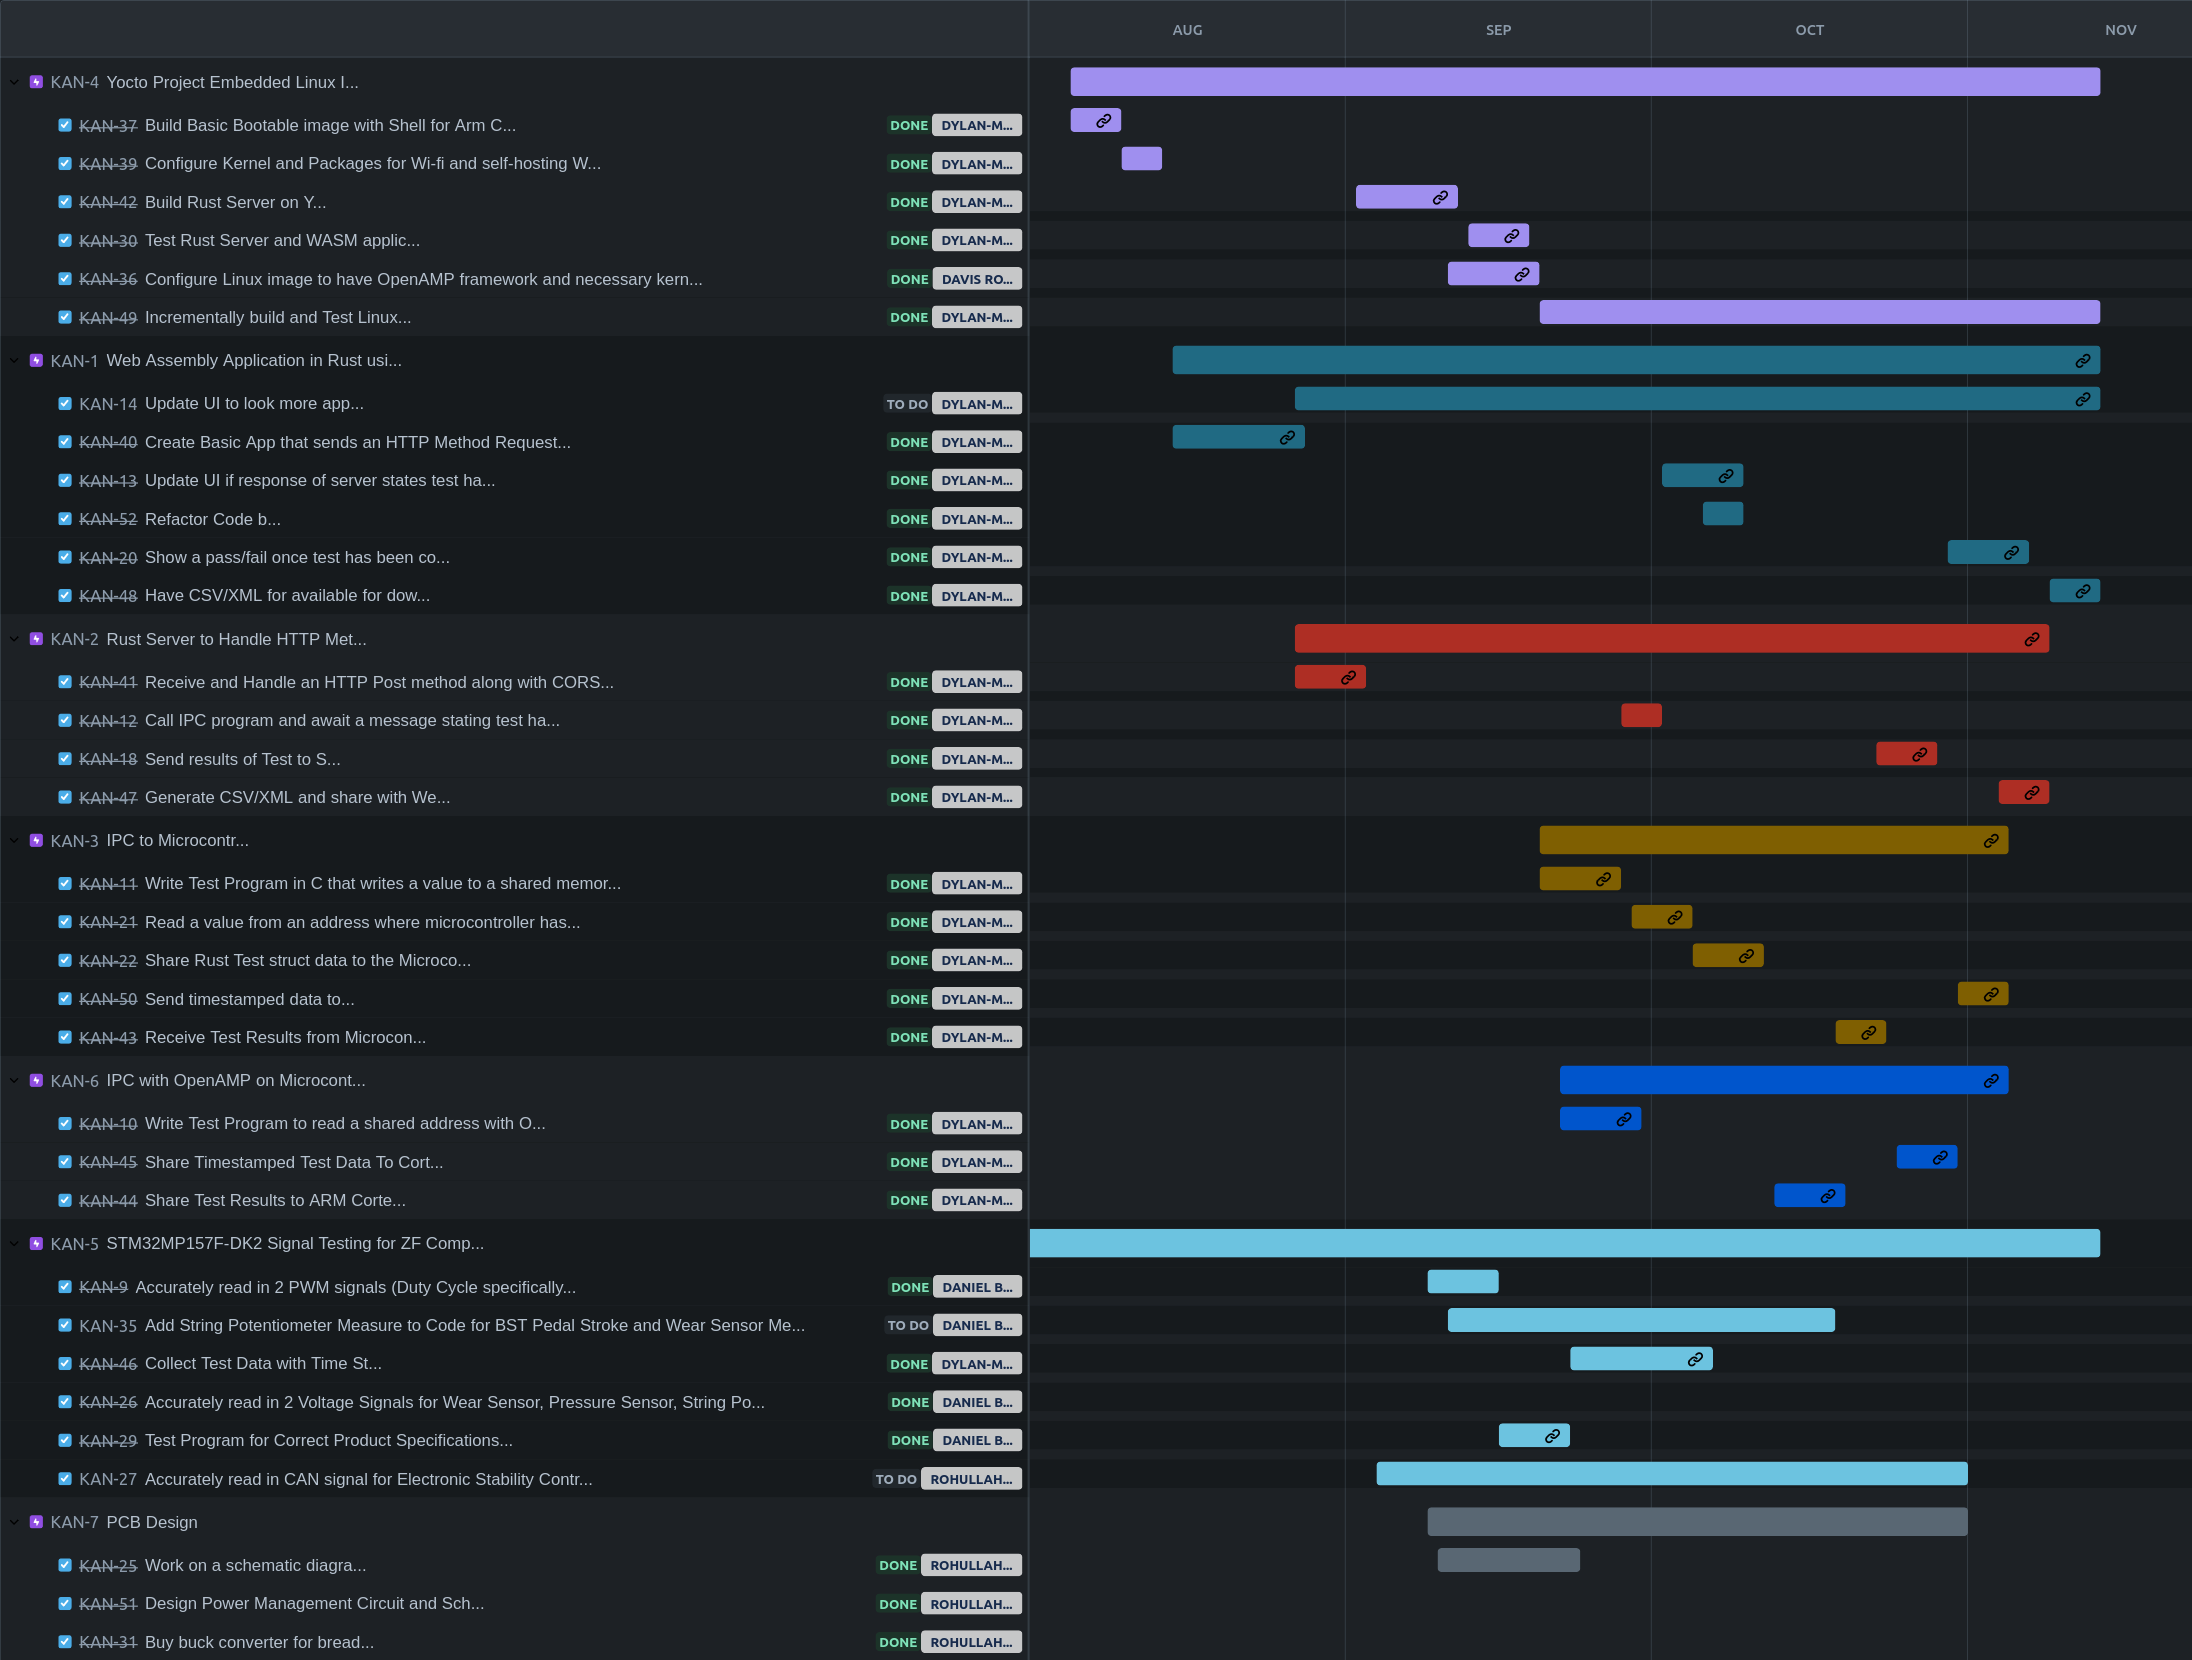
\includegraphics[height=\dimexpr\paperheight-1.5cm\relax]{assets/diagrams/gantt.png}
\end{frame}
%==============================================================================
% DESIGN AND IMPLEMENTATION SECTION: Budget Projection
%==============================================================================
\begin{frame}
  \frametitle{Budget Projection}
  \vspace{-.2025cm}
  %\includegraphics[height=\dimexpr\paperheight-1.825cm\relax]{assets/diagrams/}
\end{frame}

%==============================================================================
% DESIGN AND IMPLEMENTATION SECTION: Hardware Design
%==============================================================================
% Talk about the need and design of custom hardware (eg. simplify wiring, scale voltages for microcontroller
%   simplify connectivity, pull-up resistor network for BST)
\subsection{Hardware Design}
\begin{frame}
  \frametitle{Custom Hardware Design}
\end{frame}

%==============================================================================
% DESIGN AND IMPLEMENTATION SECTION: Cortex-M4 Firmware
%==============================================================================
\subsection{Cortex-M4 Firmware to Test Devices}
\begin{frame}
  \frametitle{Firmware to Test Brake Signal Transmitter (BST)}
\end{frame}

% CWS Test implementation
\begin{frame}
  \frametitle{Firmware to Test Continuous Wear Sensor (CWS)}
\end{frame}

% Pressure Sensor Test Implementation
\begin{frame}
  \frametitle{Firmware to Test Pressure Sensor}
\end{frame}



\end{document}
